\section{Un esempio di grafico realizzato a mano}

Supponiamo di aver misurato la capacità $C$ di un condensatore (unità di misura picofarad, pF)  in funzione della distanza tra le armature di un condensatore piano (distanza d espressa in mm). I dati sono in tabella \ref{tab:condensatore}: 

\begin{table}
\begin{center}
{
\def\arraystretch{1.5} %serve a inserire spazio bianco
\begin{tabular}{|c|c|}
\hline 
 $d\left( \si{\milli\meter}\right)$ & $C \left( \si{\pico\farad}\right)$   \\
\hline
2 & 420\\
3 &  282 \\
4 &  219 \\
5 & 182 \\
6 & 158 \\
7 &  139\\
8 &  127\\
9  & 115\\
10 & 108\\
\hline
\end{tabular}
}
\caption{Dati per il grafico capacità-distanza}
\label{tab:condensatore}
\end{center}
\end{table}
La prima cosa che notiamo, è che all'aumentare della distanza, la capacità diminuisce. Questo tipo di andamento, vedremo, è indizio (ma non è sufficiente) di una proporzionalità inversa. Ti invito a realizzare il grafico che stiamo costruendo, anche col foglio di calcolo, usando il metodo che vedremo più avanti. Vediamo quali scelte vanno fatte per il grafico.
\subsection{Disegno degli assi e titolo del grafico}
Possiamo disegnare subito gli assi lungo il bordo arancione e dare un titolo al grafico (figura \ref{fig:titoloassi})

   \begin{figure}[h!]
    \centering
    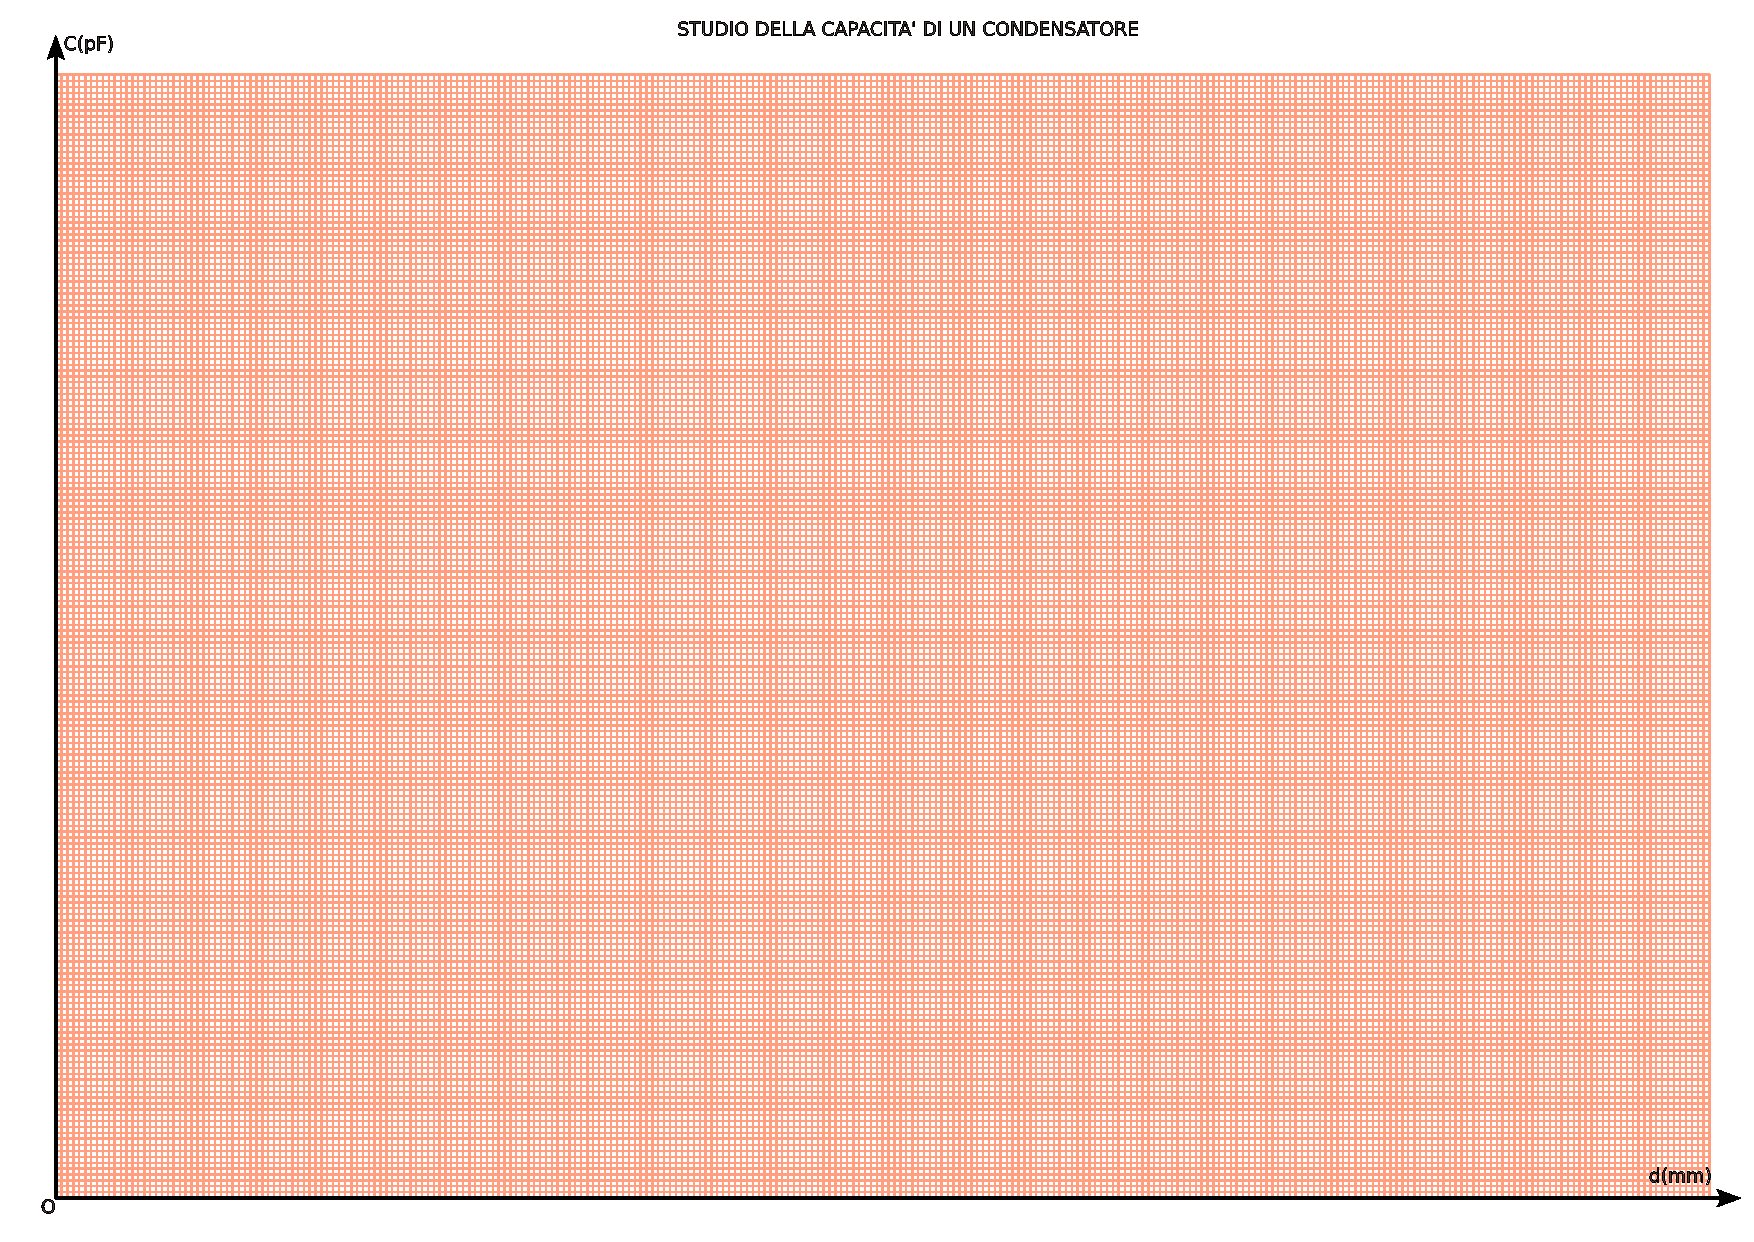
\includegraphics[width=\linewidth]{path_to_image/titoloassi.pdf} 
    \caption{Titolo e  etichette sugli assi}
    \label{fig:titoloassi}
\end{figure}  

\subsection{Scelta dei fattori di scala i valori maggiori} 
Per scegliere la scala, dobbiamo calcolare approssimativamente dove vogliamo che il grafico termini, e poiché vogliamo che venga grande, faremo in modo che i valori massimi delle due variabili capitino alla fine del foglio. Abbiamo un foglio in cui l'area arancione ha   dimensioni di $280 \times 200 $ millimetri e vogliamo che il massimo valore della distanza in tabella, ossia $\SI{10}{\milli\meter}$, capiti alla fine dell'asse X ad una distanza di circa $\SI{280}{\milli\meter}$. Dunque calcoliamo il fattore di scala sull'asse X:
\[
F_x=\frac{\SI{280}{\milli\meter}}{\SI{10}{\milli\meter}} = 28
\]
Con questo fattore potremo inserire ogni dato della prima colonna sul grafico moltiplicandolo per $F_x$. Per esempio, il valore $\SI{2}{\milli\meter}$ andrà inserito sul punto dell'asse X di ascissa $28\times\SI{2}{\milli\meter} = \SI{56}{\milli\meter}$. Analogamente, il fattore di scala sull'asse Y è:
\[
F_y = \frac{\SI{200}{\milli\meter}}{\SI{420}{\pico\farad}} = \SI{0,476}{\milli\meter\per\pico\farad}.
\] 

E' sempre meglio approssimare per difetto i fattori di scala, altrimenti i valori massimi della tabella, potrebbero uscire dai bordi del foglio (dalla parte colorata).
Effettuando i calcoli, otteniamo per i dati sull'asse X:
\begin{equation*}
\begin{aligned}
\SI{2}{\milli\meter} \times 28 &= \SI{56}{\milli\meter}  \\
\SI{3}{\milli\meter}  \times 28 &= \SI{84}{\milli\meter}  \\
\SI{4}{\milli\meter}  \times 28 &= \SI{112}{\milli\meter}   \\
\SI{5}{\milli\meter}  \times 28 &= \SI{140}{\milli\meter}  \\
\SI{6}{\milli\meter}  \times 28 &= \SI{168}{\milli\meter}   \\
\SI{7}{\milli\meter}  \times 28 &= \SI{196}{\milli\meter}  \\
\SI{8}{\milli\meter}  \times 28 &= \SI{224}{\milli\meter}  \\
\SI{9}{\milli\meter}  \times 28 &= \SI{252}{\milli\meter}  \\
\SI{10}{\milli\meter}  \times 28 &= \SI{280}{\milli\meter}  \\
\end{aligned}
\end{equation*}
Facciamo anche i calcoli per i dati da inserire sull'asse Y:

\[
\begin{array}{rcl}
\SI{420}{\pico\farad} \times \SI{0.476}{\milli\meter\per\pico\farad} &=& \SI{199.92}{\milli\meter} \\
\SI{282}{\pico\farad} \times \SI{0.476}{\milli\meter\per\pico\farad} &=& \SI{134.232}{\milli\meter} \\
\SI{219}{\pico\farad} \times \SI{0.476}{\milli\meter\per\pico\farad} &=& \SI{104.244}{\milli\meter} \\
\SI{182}{\pico\farad} \times \SI{0.476}{\milli\meter\per\pico\farad} &=& \SI{86.632}{\milli\meter} \\
\SI{158}{\pico\farad} \times \SI{0.476}{\milli\meter\per\pico\farad} &=& \SI{75.208}{\milli\meter} \\
\SI{139}{\pico\farad} \times \SI{0.476}{\milli\meter\per\pico\farad} &=& \SI{66.164}{\milli\meter} \\
\SI{127}{\pico\farad} \times \SI{0.476}{\milli\meter\per\pico\farad} &=& \SI{60.452}{\milli\meter} \\
\SI{115}{\pico\farad} \times \SI{0.476}{\milli\meter\per\pico\farad} &=& \SI{54.74}{\milli\meter} \\
\SI{108}{\pico\farad} \times \SI{0.476}{\milli\meter\per\pico\farad} &=& \SI{51.408}{\milli\meter} \\
\end{array}
\]
Ovviamente, questi valori devono essere arrotondati per difetto al millimetrio più vicino (il foglio permette al massimo di tracciare i millimetri). Queste due tabelle dei calcoli, non vanno riportate sul foglio di relazione ma solo sui propri appunti. Quello che ci interessa sono i numeri finali (i millimetri). Riportiamo in fine, i dati sul grafico (figura \ref{fig:graficomanuale}) dove abbiamo anche tracciato (ad occhio) una linea di tendenza. 
 
    \begin{figure}[h!]
    \centering
    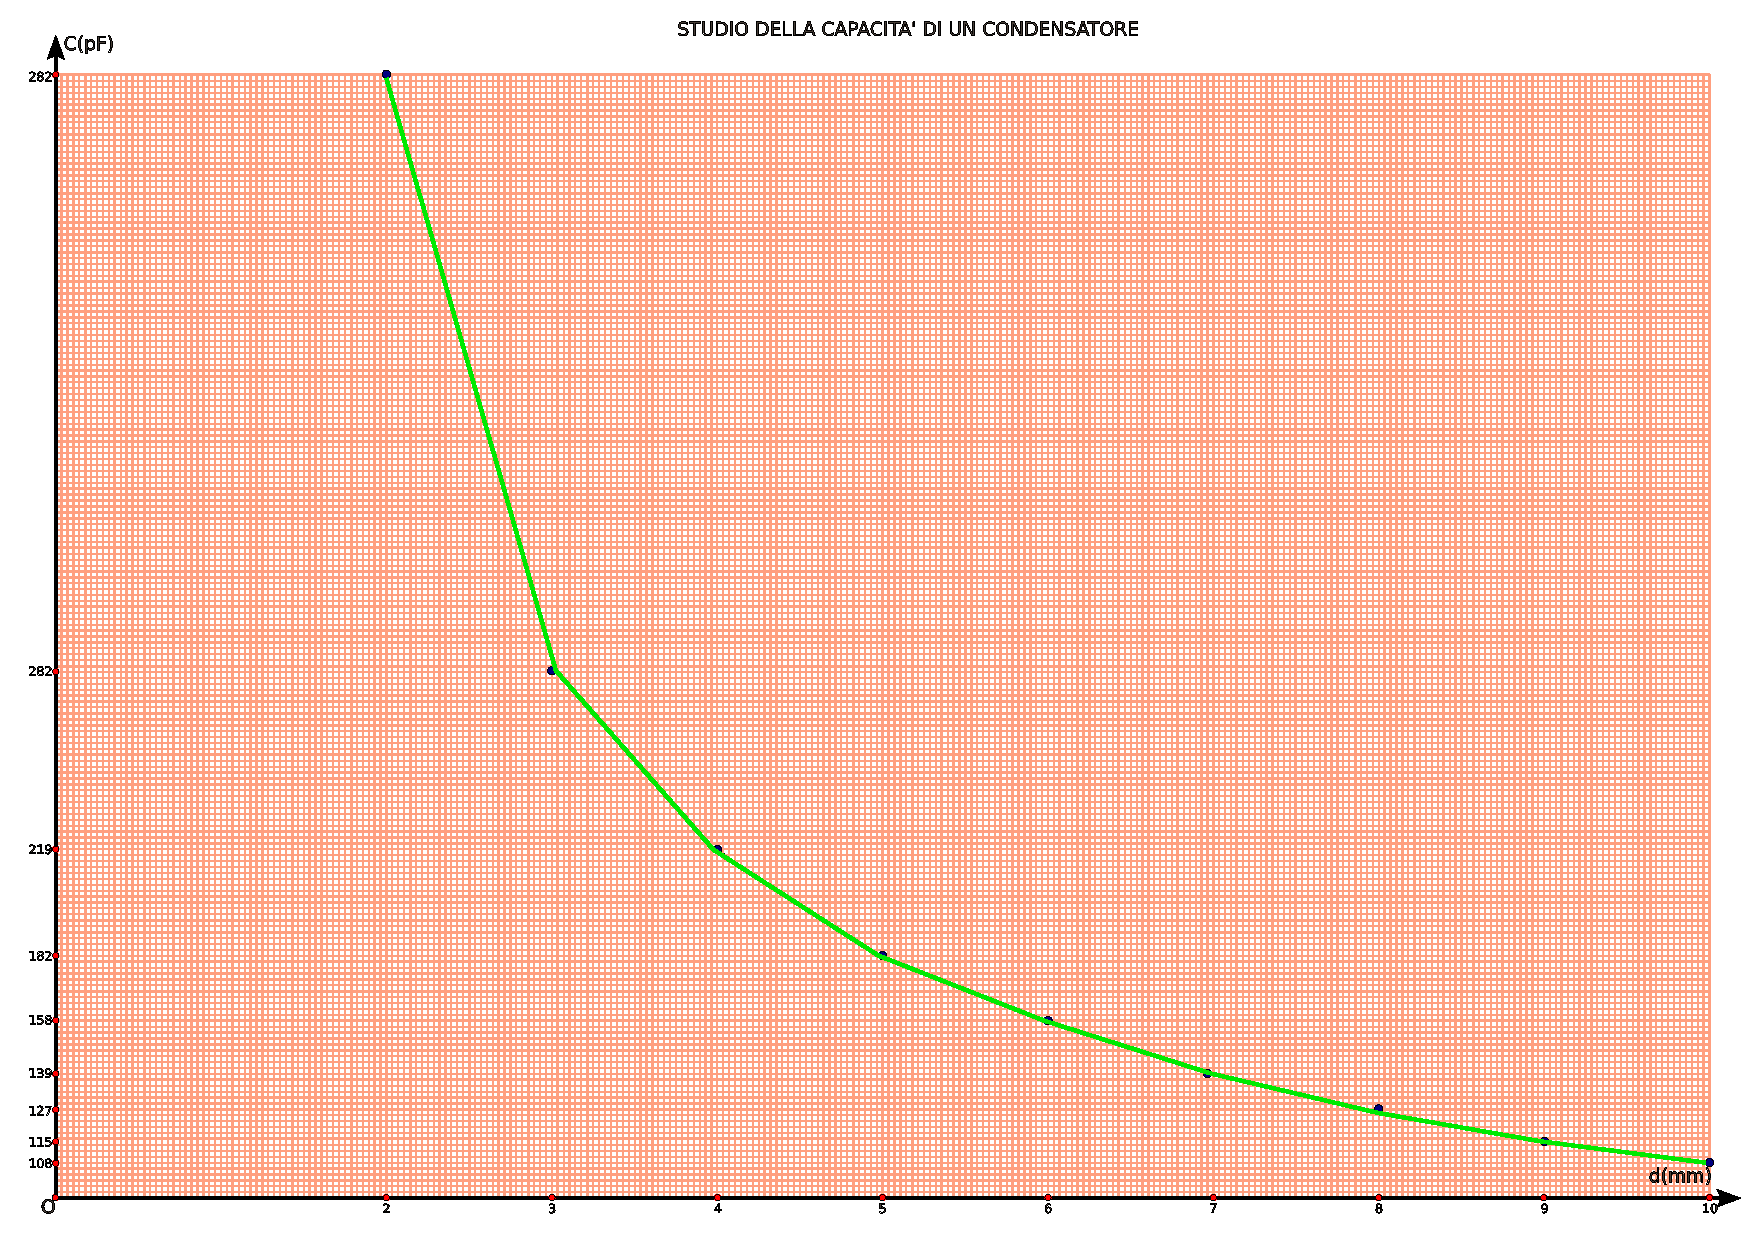
\includegraphics[width=\linewidth]{path_to_image/graficomanuale.pdf} 
    \caption{Grafico su carta millimetrata.}
    \label{fig:graficomanuale}
\end{figure} 



